\subsection{Preduction of missidentified Quark/Gluon Jets}\label{sec:tauFakeBackground}
One of the most important backgrounds is induced by quark or gluon jets that are mistaken to originate from hadronic $\tau$
decays. Even though sophisticated $\tau$ identification algorithms are in place the abundance of such jets at proton--proton
collisions lead to a leading contribution of misidentified jets (fakes) to the overall background.\\
We derive this contribution using the tight to loose ratio method. Where loose candidates are any AK5 jets that satisfy:
\begin{itemize}
\item $p_T > 15$ GeV
\item $|\eta| < 2.3$
\item charge == 1
\item muon and electron discrimination
\item isolation by leading pion
\end{itemize}
The addition of the TaNC WP with an expected fake rate of $1\%$ yields the full $\tau$ object definition and the tight
selection.
\begin{figure}[hbtp]
  \subfigure[]{\label{fig:tauTightToLoose}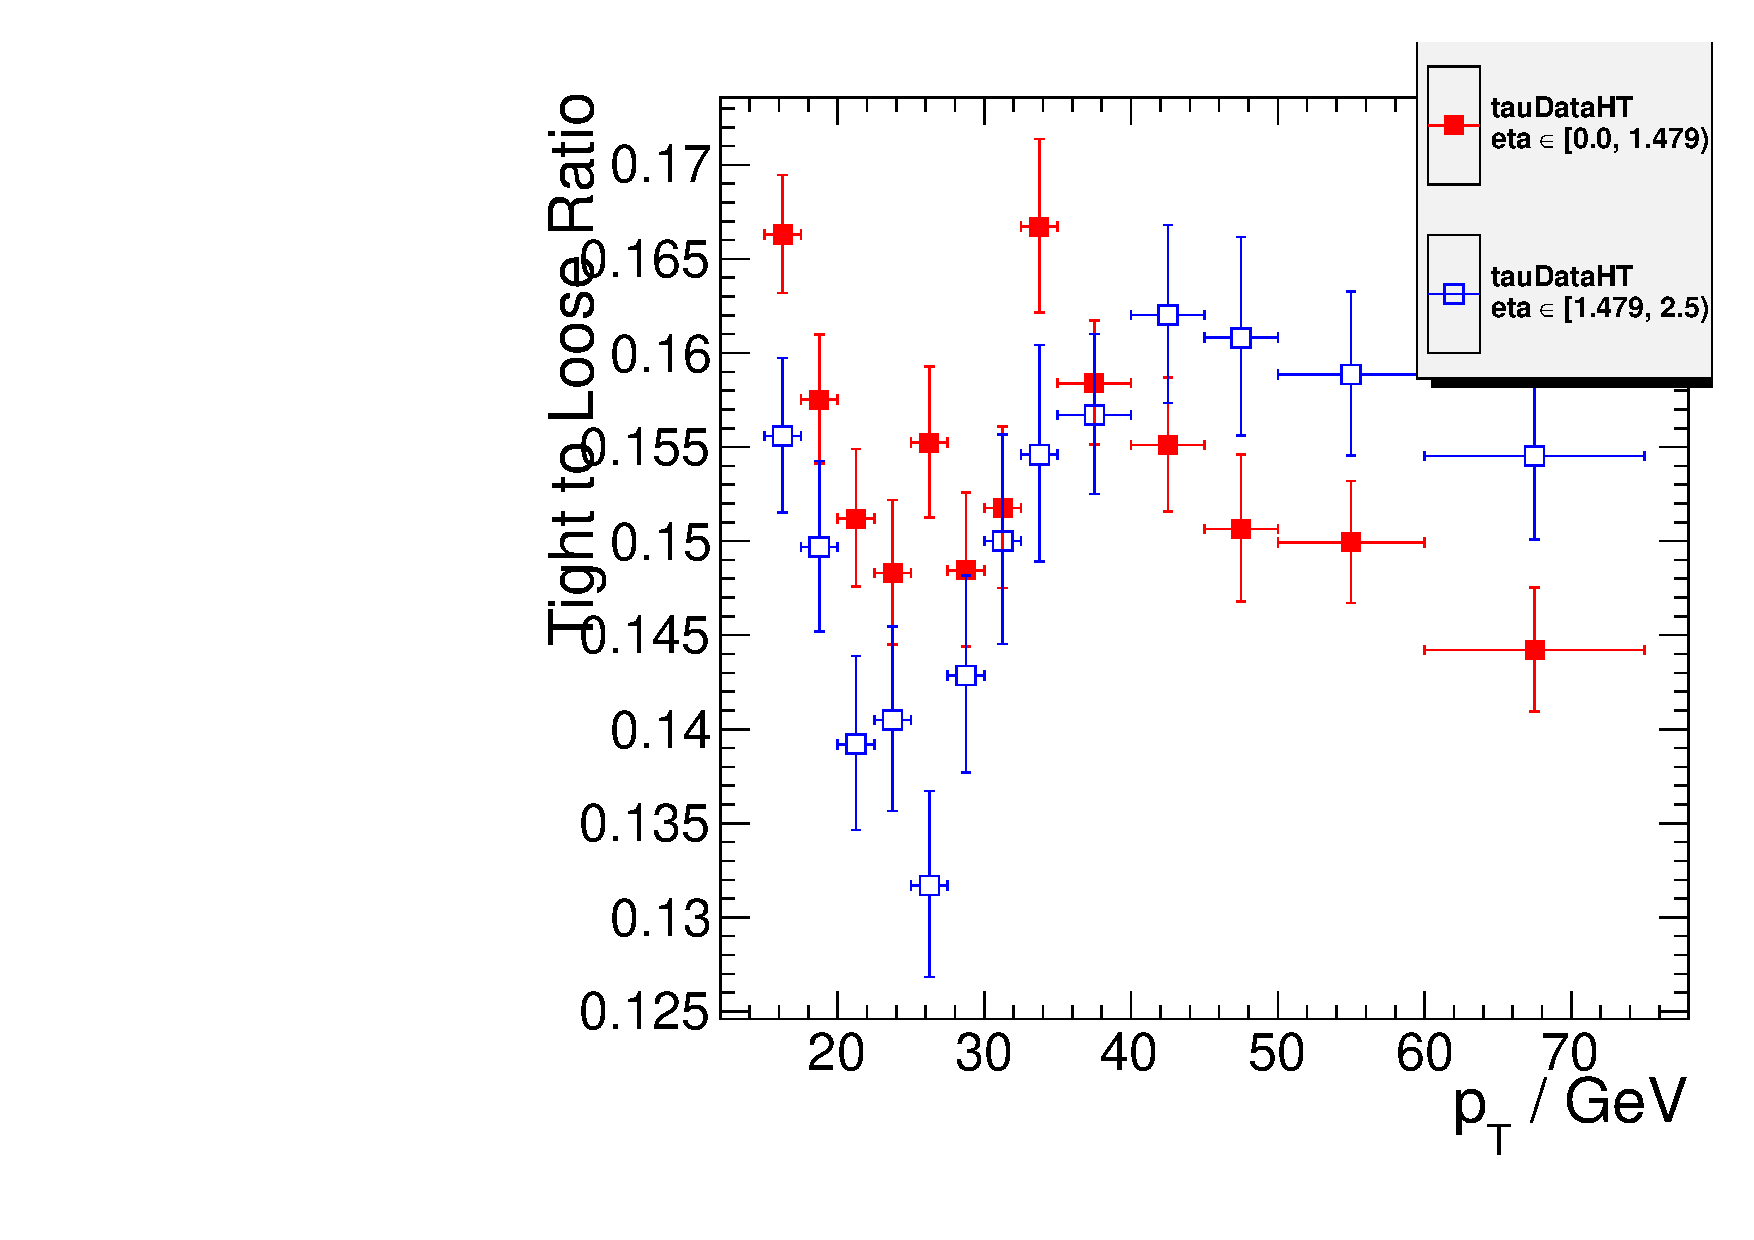
\includegraphics[width=0.79\textwidth]{plots/pt_tauDataHT.pdf}}\hfill
  \caption{Ratio of jets passing the tight to jets passing the loose definition in the region of $HT > 250$ GeV and $\MET <
    20$ GeV. Filled points denote this ration in the barrel and open points in the endcap region.}
\end{figure}
In a Background dominated region ($HT > 250$ GeV and $\MET < 20$ GeV) the ratio of the numer of tight candidates to those
passing the loose definition is calculated in bins of transverse momentum and pyseudo rapidity as shown in
Fig. \ref{tauTightToLoose}.\\

A prediction of the number of misidentified jets can later be derived by selecting jets that pass the loose but not the tight
selection criteria in the signal region and applying for the measured tight to loose ration $f(p_T, |\eta|)$ a weight of $\frac{f}{1-f}$.
